\section{Auswertung}
\label{sec:Auswertung}

\subsection{Bestimmung von Widerständen mittels Wheatstone-Brücke}
Die verschiedenen Werte für die Widerstände $R_3$, $R_4$ und $R_2$, die zur Berechnung des Widerstandes $R_X$
nötig sind, befinden sich in Tabelle \ref{taba}. Dabei beziehen sich die ersten drei Zeilen auf den Widerstand
$R_{X1}$ und die letzten drei auf den Widerstand $R_{X2}$.
\begin{table}\caption{Die Länge der Zylinder und die Spannung mit den jeweiligen Zeitenpunkten der Ausschläge.}
\label{taba}
\centering
\sisetup{round-mode = places, round-precision=2, round-integer-to-decimal=true}
\begin{tabular}{S[]S[]S[]S[]S[]} 
\toprule
{$l/ \si{\milli\meter}$} & {$U_1/ \si{\volt}$} & {$t_1/ \si{\micro\second}$} & {$U_2/ \si{\volt}$} & {$t_2/ \si{\micro\second}$}\\
\midrule
120.8 & 1.29 & 0.6 & 0.17 & 88.7\\
102.3 & 1.27 & 0.5 & 0.2 & 76.5\\
80.5 & 1.33 & 0.6 & 0.76 & 59.8\\
40.4 & 1.33 & 0.5 & 1.34 & 30.2\\
31.1 & 1.29 & 0.5 & 1.37 & 23.8\\
\bottomrule
\end{tabular}\end{table}
Die gesuchten Widerstände lassen sich daraus mit Gleichung \eqref{eqn:a_r} berechnen.
Für den ersten Widerstand ergibt sich
\begin{equation*}

\end{equation*}

\subsection{Bestimmung von Kapazitäten mittels Kapazitätsmessbrücke}

\subsection{Bestimmung von Induktivitäten mittels Induktivitätsmessbrücke}

\subsection{Bestimmung von Induktivitäten mittels Maxwell-Brücke}

\subsection{Bestimmung der Frequenzabhängigkeit der Brückenspannung mittels Wien-Robinson-Brücke}

\begin{figure}
 \centering
 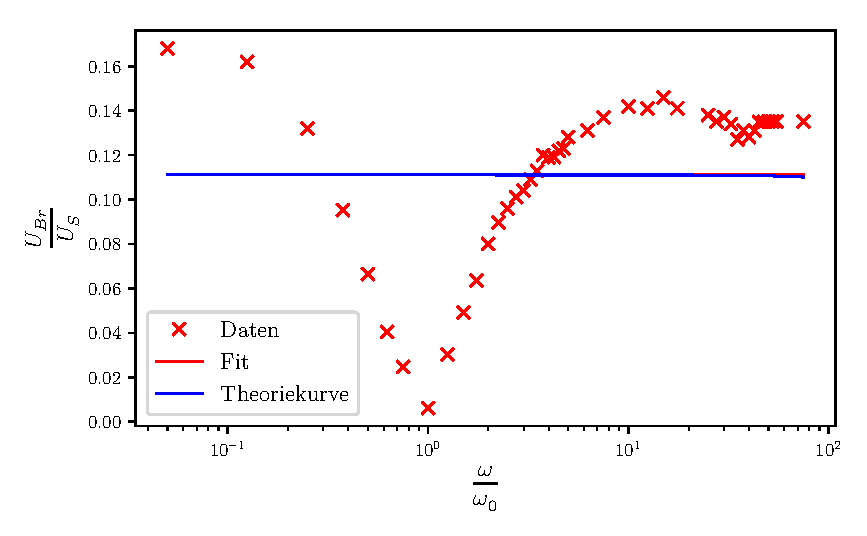
\includegraphics{plot1.pdf}
 \caption{Plot}
 \label{fig:plot}
\end{figure}

\subsection{Bestimmung des Klirrfaktors}